\documentclass[12pt]{article}

\usepackage{graphicx}
\usepackage{titlesec}
\usepackage{xcolor}
\usepackage{enumitem}
\usepackage{subcaption}
\usepackage{float}
\usepackage{placeins}
\usepackage[none]{hyphenat}
\usepackage[most]{tcolorbox}
\usepackage[italian]{babel}
\usepackage[a4paper, margin=75pt]{geometry}
\usepackage[colorlinks=true, linkcolor=black]{hyperref}

\graphicspath{{images/}}
\setlist{itemsep=2pt}
\definecolor{greenpastel}{RGB}{180, 230, 180}
\tcbset{
  myboxstyle/.style={
    colback=white,
    coltitle=black,
    fonttitle=\bfseries,
    colframe=greenpastel
  }
}

\newcounter{definition}[section]
\renewcommand{\thedefinition}{\thesection.\arabic{definition}}
\newtcolorbox{definition}[1][]{
  myboxstyle,
  colframe=greenpastel,
  boxed title style={colback=greenpastel},
  before title={\refstepcounter{definition}},
  title={Definizione \thedefinition: #1}
}


\titleformat{\section}
  [block]
  {\raggedleft\LARGE\bfseries}
  {\textcolor{gray}{\scalebox{5}{\thesection}}}
  {0pt}
  {\\[3pt]}

\titlespacing*{\section}
  {0pt}   % rientro sinistro
  {0pt}   % spazio prima della sezione
  {30pt}  % spazio dopo la sezione


\begin{document}
% --- Copertina ---
\begin{titlepage}
\centering

% --- Logo Sapienza ---

\includegraphics[width=0.95\textwidth]{logo_sapienza.png}

\vspace*{\stretch{0.2}}

% --- Dati Sapienza ---
{\LARGE "Sapienza" Università di Roma}\\[3pt]
{\Large Ingegneria dell'Informazione, Informatica e Statistica}\\[3pt]
{\large Dipartimento di Informatica}\\[3pt]

% --- Spazio vuoto ---
\vspace*{\stretch{1}}

% --- Titolo ---
\hrulefill\\
\vspace{15pt}
\textbf{\huge Programmazione WEB}\\
\vspace{7pt}
\hrulefill\\

% --- Spazio vuoto ---
\vspace*{\stretch{2}}

% --- Autore ---
\textit{\Large Autore}\\[3pt]
{\Large Vincenzo Bova}\\

% --- Spazio vuoto ---
\vspace*{\stretch{1}}

% --- Data ---
{\large A.A. 2025/2026}\\
\end{titlepage}

% --- Indice ---
\newpage
\setcounter{tocdepth}{2}
\tableofcontents

% --- Introduzione a Git ---
\newpage
\section{Introduzione a Git}
\subsection{Sistemi di versionamento}
Durante lo sviluppo di un progetto c'è spesso la necessità di effettuare revisioni, correzioni o modifiche ai file che lo compongono.
\begin{figure}[H]
\centering

\includegraphics[width=0.5\textwidth]{introduzione_a_git/no_git_example.png}
\end{figure}
Gestire ciò creando ogni volta nuovi file, tuttavia, comporta evidenti problemi:
\begin{itemize}
\item \textbf{Duplicazione del contenuto:} che rende il sistema inefficiente e aumenta la difficoltà nel mantenere integrità;
\item \textbf{Assenza di Naming Convention:} che rende impossibile risalire ad uno storico delle modifiche;
\item \textbf{Autori incerti};
\item \dots
\end{itemize}
\begin{samepage}
Per ovviare a ciò sono stati creati i \textbf{sistemi di versionamento} (git, csv, mercurial, svn\dots), i quali offrono vari benefici:
\begin{itemize}
\item \textbf{Gestione delle versioni:} il sistema si occupa automaticamente di etichettare le varie versioni in modo consistente;
\item \textbf{Tracciamento delle mofiche:} è possibile accedere ad uno storico delle modifiche effettuate;
\item \textbf{Presenza di metadati:} ogni modifica ha un autore, una data\dots;
\item \textbf{Creazione di linee di sviluppo parallele:} è possibile creare una versione parallela del codice per non modificare la versione principale, e poi riunirle integrando i cambiamenti;
\item \textbf{Sincronizzazione tra computer:} il sistema consente di mantenere il progetto allineato tra più computer.
\end{itemize}
\end{samepage}

\subsection{Git}
Git è un sistema di versionamento distribuito e veloce, creato nel 2005 e capace di gestire progetti di grandi dimensioni.
Si basa su un design semplice e utilizza DAG (\textit{Directed Acyclic Graph}) e Merkle trees come strutture dati.
\begin{definition}[Repository]
È un insieme di commit, branch e tag.\\
Per semplicità assumiamo che un progetto equivale ad un repository.
\end{definition}
\begin{definition}[Working copy]
È l'insieme dei file tracciati nella copia locale del repository.\\
Quando creiamo un nuovo file non sarà ancora tracciato e bisognerà quindi aggiungerlo, quando invece modifichiamo un file già tracciato (\textit{update}) stiamo aggiornando la working copy.
\end{definition}

\subsubsection{Commit}
Un commit è un'istantanea del repository in un determinato momento.\\
Viene identificato dallo \textbf{SHA1} del commit stesso e contiene diversi campi:
\begin{itemize}
\item data + autore, data + commiter
\item commento \textbf{obbligatorio}
\item 0,1 o più genitori
\item tree: hash di tutti i file nel commit
\end{itemize}
\begin{minipage}{\textwidth}
In particolare il commit può contenere un sottoinsieme delle modifiche (anche ad un singolo file), le quali devono essere aggiunte alla staging area dei cambiamenti.
\begin{figure}[H]
\centering
\begin{subfigure}{0.49\textwidth}
\centering
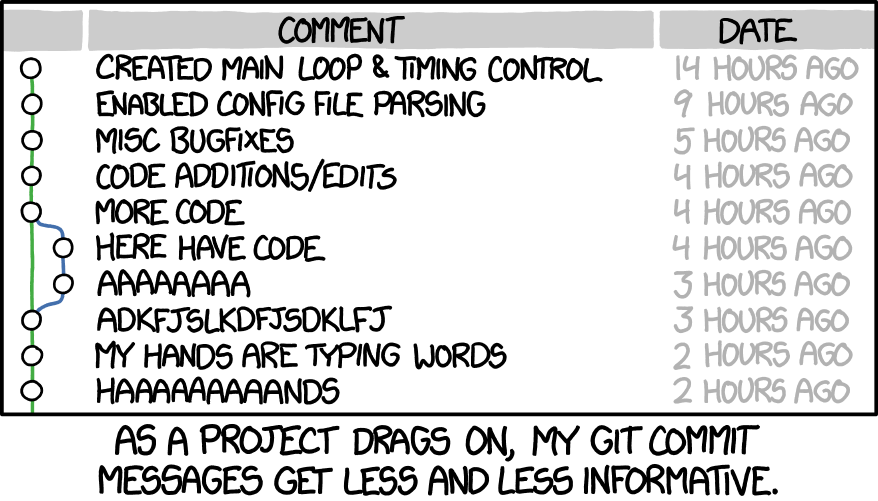
\includegraphics[height=4cm]{introduzione_a_git/git_commit.png}
\end{subfigure}
\hfill
\begin{subfigure}{0.49\textwidth}
\centering
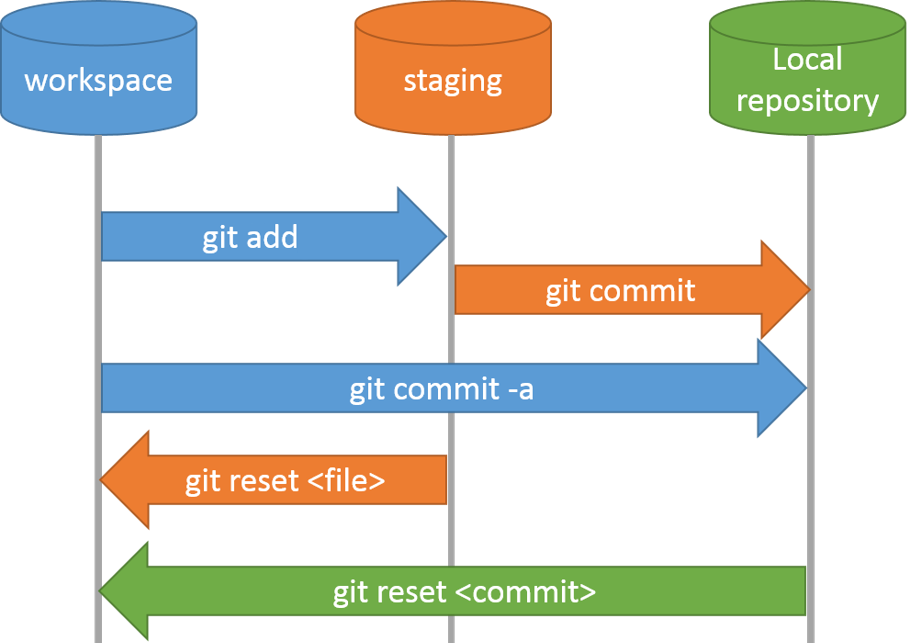
\includegraphics[height=4cm]{introduzione_a_git/git_commit_staging.png}
\end{subfigure}
\end{figure}
\end{minipage}

\subsubsection{Branch}
Un branch è una linea di sviluppo, composta da un insieme ordinato di commit collegati in un DAG, il quale inizia dal primo commit del repository e punta all'ultimo commit.\\
Grazie ai branch è possibile \textbf{lavorare parallelamente} a più versioni del progetto.
\begin{figure}[H]
\centering
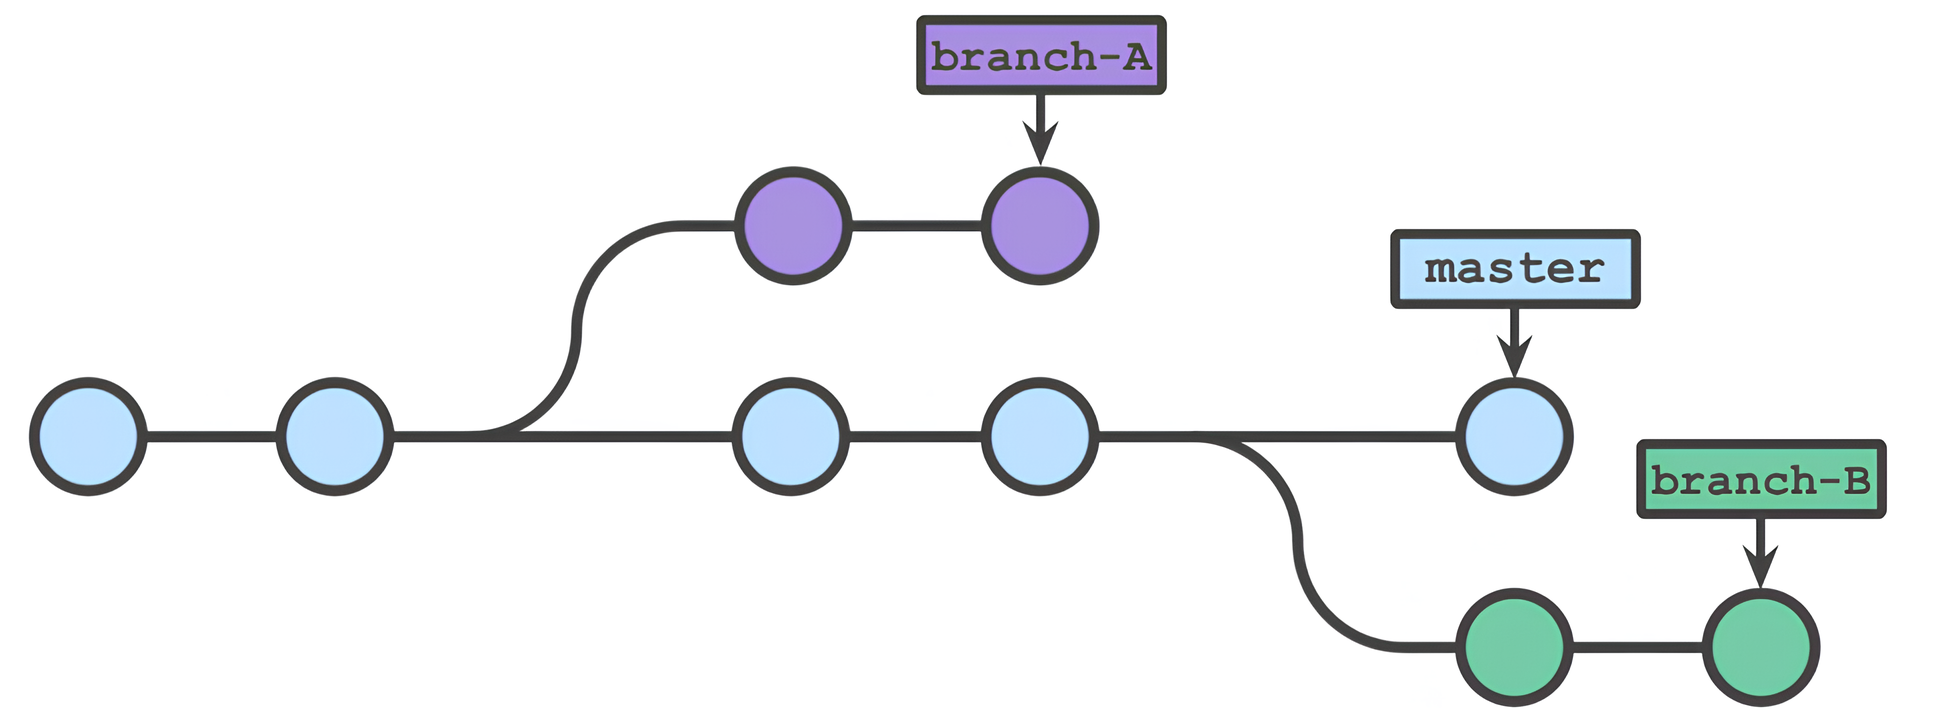
\includegraphics[width=0.7\textwidth]{introduzione_a_git/branch.png}
\end{figure}

\subsubsection{HEAD}
L'HEAD è un puntatore alla posizione attuale rispetto alla storia del repository e può essere aggiornato tramite il comando \textit{checkout}.\\
Solitamente l'HEAD punta ad un branch o ad un tag, qualora invece puntasse ad un commit si parlerebbe di \textbf{Detached HEAD}. Quando ci si trova in questo stato i commit fatti non vengono inseriti in alcun branch, rischiando quindi di andare persi.
\begin{figure}[H]
\centering
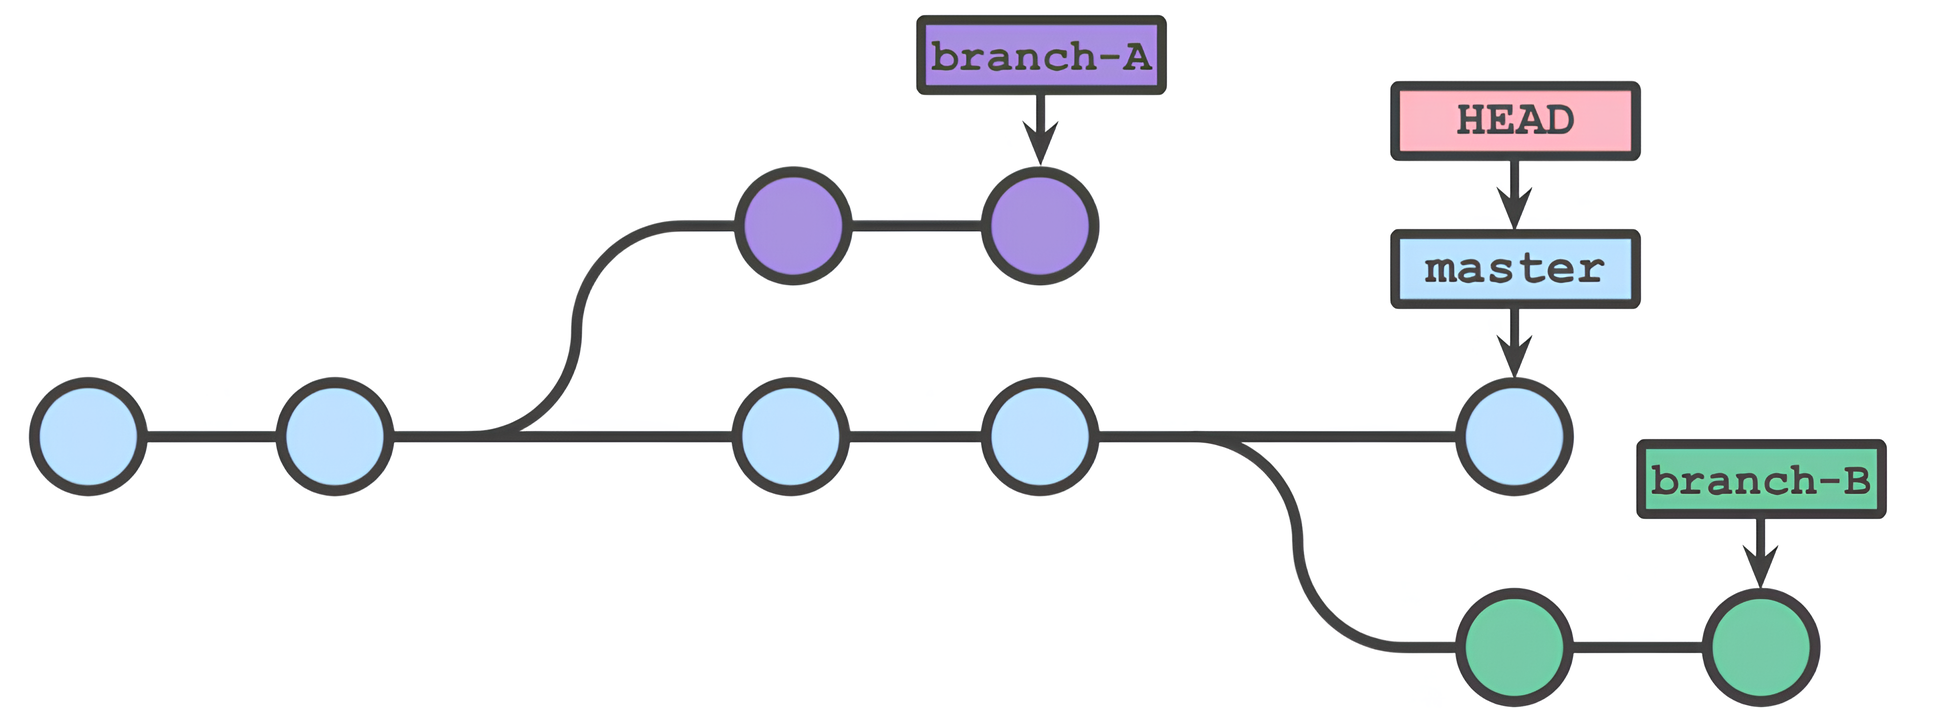
\includegraphics[width=0.7\textwidth]{introduzione_a_git/branch_head.png}
\end{figure}

\subsubsection{Tag}
Un tag è un'etichetta per un commit e viene solitamente usato per segnare versioni importandi di un progetto (es. \textit{v1.0.0}, \textit{release-2025-09}).

\subsubsection{Remotes}
Sono dei riferimenti ai branch in repository remoti. Il nome predefinito è \texttt{origin} e vengono visualizzati nel formato \texttt{<remote>/<branch>} (es. \texttt{origin/main}).\\
In particolare definiamo come \textbf{tracking branch} un branch locale che tiene traccia di un branch remoto, facilitando l'uso dei comandi \texttt{git push} e \texttt{git pull}.

\subsubsection{Merge}
Il merge è un'operazione che fonde i cambiamenti apportati in due branch distinti, facendo in modo che il branch di destinazione contenga entrambi i cambiamenti e che quello di origine rimanga immutato.\\
Quando questa operazione viene eseguita tramite comando, Git determina in maniera autonoma quale tipo di merge sia più appropriato, basandosi sulla relazione tra i due branch e sullo storico dei loro commit.\\
In particolare esistono quattro tipologie di merge:
\begin{itemize}
\item \textbf{Fast forward:}
\begin{itemize}
\item \textit{Condizione:} il branch di origine è diretto discendente di HEAD.
\item \textit{Azione:} Git sposta solo il puntatore di HEAD in avanti. 
\item \textit{Risultato:} nessun nuovo merge commit. 
\end{itemize}
\item \textbf{Merge commit:}
\begin{itemize}
\item \textit{Condizione:} i branch divergono e hanno sviluppi indipendenti;
\item \textit{Azione:} Git combina le modifiche dei due branch, creando un nuovo commit;
\item \textit{Risultato:} viene creato un merge commit con due genitori;
\end{itemize}
\item \textbf{Rebase:}
\begin{itemize}
\item \textit{Condizione:} si vuole aggiorare un branch basandolo su un altro, riscrivendo lo storico;
\item \textit{Azione:} Git ricrea ogni commit non in comune tra i due branch; 
\item \textit{Risultato:} la storia del branch diventa lineare, senza merge commit intermedi. 
\end{itemize}
\item \textbf{Three way:}
\begin{itemize}
\item \textit{Condizione:} storie divergenti (commit unici su entrambi i branch);
\item \textit{Punti di confronto:}
\begin{enumerate}
\item Base comune (Ancestor);
\item Versione locale (HEAD);
\item Versione remota (Branch);
\end{enumerate}
\item \textit{Azione:} Git crea un nuovo snapshot combinando le modifiche;
\item \textit{Risultato:} Viene creato un merge commit.
\end{itemize}
\end{itemize}

\subsection{Comandi Git}
Per interfacciarsi con Git vengono messi a disposizione dal sistema diversi comandi:
\begin{itemize}
\item \texttt{git init:} inizializza un repository creando una subdirectory .git all'interno della directory corrente; 
\item \texttt{git status:} mostra lo stato attuale del repository (file tracciati, file modificati, file nello staging, file non tracciati);
\item \texttt{git diff:} mostra le differenze tra working directory, staging e commit;
\item \texttt{git add <file>:} aggiunge un file alla staging area (\texttt{git add .} per aggiungere tutti i file modificati);
\item \texttt{git commit -m "Messaggio":} crea un commit, registrando le modifiche aggiunte con \texttt{git add} nella cronologia del repository;
\item \texttt{git log:} mostra la lista dei commit effettuati;
\item \texttt{git branch <nome>:} crea un nuovo branch con il nome indicato, ma \textbf{non ci si sposta};
\item \texttt{git checkout <nome>:} passa ad un branch esistente spostando l'HEAD;
\item \texttt{git checkout -b <nome>:} crea un nuovo branch con il nome indicato, per poi \textbf{spostarsi} su quest'ultimo (\texttt{git checkout -b <nome>} = \texttt{git branch <nome>} + \texttt{git checkout <nome>});
\item \texttt{git fetch:} scarica gli aggiornamenti (commit, branch) dal repository remoto, \textbf{senza merge} col tuo branch;
\item \texttt{git merge <branch>:} unisce la cronologia del branch in cui ci si trova con quella del branch specificato;
\item \texttt{git pull:} scarica gli aggiornamenti (commit, branch) dal repository remoto, \textbf{facendo merge} col tuo branch (\texttt{git pull} = \texttt{git fetch} + \texttt{git merge});
\item \texttt{git push:} invia i commit locali al repository remoto, aggiornando il branch remoto corrispondente; 
\end{itemize}

\begin{samepage}
\subsection{Git flow}
Con il termine Git flow intendiamo un modello di branching rigido per la gestione di rilasci e cicli di sviluppo definiti.\\
Il suo scopo è quello di separare gli ambienti di produzione, sviluppo, funzionalità e correzioni, attraverso i seguenti branch:
\begin{itemize}
\item \texttt{main/master}
\begin{itemize}
\item \textbf{Contenuto:} solo codice stabile, testato e rilasciato.;
\item \textbf{Checkout da:} \texttt{release-*} o \texttt{hotfix-*};
\item \textbf{Tag:} ogni merge riceve un tag di versione (es. \textit{v1.0});
\end{itemize}
\item \texttt{develop}
\begin{itemize}
\item \textbf{Contenuto:} cronologia completa delle funzionalità di sviluppo;
\item \textbf{Checkout da:} \texttt{feature-*};
\item \textbf{Merge in:} \texttt{release-*}
\end{itemize}
\item \texttt{feature-*}
\begin{itemize}
\item \textbf{Scopo:} lavoro isolato su una nuova funzionalità;
\item \textbf{Checkout da:} \texttt{develop};
\item \textbf{Merge in:} \texttt{develop};
\item \textbf{Regola:} non interagisce mai con \texttt{main};
\end{itemize}
\item \texttt{release-*}
\begin{itemize}
\item \textbf{Scopo:} preparazione per il prossimo rilascio;
\item \textbf{Checkout da:} \texttt{develop};
\item \textbf{Attività:} Solo bug fixing minori e aggiornamento metadata (numero di versione);
\item \textbf{Doppio merge in:} \texttt{main} per il rilascio in produzione e \texttt{develop} per preservare le correzioni;
\end{itemize}
\item \texttt{hotfix-*}
\begin{itemize}
\item \textbf{Scopo:} Correzione immediata di bug critici trovati nel \texttt{main};
\item \textbf{Checkout da:} \texttt{main}
\item \textbf{Doppio merge in:} \texttt{main} per deployare subito la correzione e \texttt{develop} per garantire che il bug non riappaia in futuro;
\end{itemize}
\end{itemize}
\end{samepage}

\newpage
\subsection{Gestione dei conflitti}
Immaginiamo un contesto in cui tre sviluppatori lavorano allo stesso progetto:
\begin{itemize}
\item \textbf{Marco} (\texttt{fix-data-leakage}): si accorge di una falla critica nel preprocessing del dataset. Ha fatto 4 commit sul suo branch;
\item \textbf{Luca} (\texttt{update-rules-parser}): ha aggiornato il parser delle regole della community, modificando gli \textbf{stessi file} di preprocessing toccati da Marco. Ha fatto 3 commit sul suo branch;
\item \textbf{Voi} (\texttt{main}): effettuate il merge del lavoro di Marco senza problemi e ora dovete unire il lavoro di Luca.
\end{itemize}
Nel momento in cui proverete ad effettuare il secondo merge, Git non ve lo consentirà, mettendo in pausa il merge e marcando i file in conflitto nel seguente modo:
\begin{code}
  <<<<<<< HEAD
  # Codice sul branch main
  =======
  # Codice sul branch update-rules-parser
  >>>>>>> update-rules-parser
\end{code}
A questo punto sarà necessario risolvere i conflitti tramite l'interfaccia grafica aperta dal comando \texttt{git mergetool},
oppure manualmente aprendo ogni file, rimuovendo i marcatori di confitto e rieffettuando il commit.

\subsection{Annullamento delle operazioni}
\begin{itemize}
\item \textbf{Annulare in staging:} dopo aver eseguito \texttt{git add}, qualora non si volesse più committare il file, è possibile rimuoverlo dall'area di staging tramite il comando \texttt{git reset HEAD -- <file>};
\item \textbf{Annullare modifiche locali:} dopo aver modificato un file, è possibile scartare le modifiche e ripristinare quest'ultimo alla versione dell'ultimo commit tramite il comando \texttt{git checkout -- <file>};
\item \textbf{Annullare un commit pubblicato:} dopo aver eseguito un commit ed averlo pubblicato, è possibile annullarlo tramite il comando \texttt{git revert <hash-commit>};
\item \textbf{Annullare un commit locale:} dopo aver eseguito un commit, qualora quest'ultimo non sia ancora stato pubblicato, è possibile annullarlo tramite il comando\\\texttt{git reset <--soft|--hard> HEAD\raisebox{-0.5ex}{\~{}}1}, dove:
\begin{itemize}
\item \texttt{--soft} rimuove l'ultimo commit mantenendo le modifiche nell'area di staging;
\item \texttt{--hard} rimuove l'ultimo commit cancellando completamente le modifiche;
\item \texttt{HEAD\raisebox{-0.5ex}{\~{}}1} indica il commit direttamente precedente ad HEAD (\texttt{HEAD\raisebox{-0.5ex}{\~{}}3} indica il 3°, etc\dots); 
\end{itemize}
\item \textbf{Riscrivere l'ultimo commit:} per rimpiazzare l'ultimo commit con uno nuovo è possibile utilizzare il comando \texttt{git commit --amend}.
\end{itemize}

% --- HTTP ---
\newpage
\section{HTTP}
L'\textbf{HyperText Transfer Protocol} (HTTP) è un protocollo a livello di applicazione nello stack di protocolli Internet, progettato per la trasmissione di informazioni.\\
La variante sicura è \textbf{HTTPS} e nel 2022 è stato pubblicato HTTP/3.\\
L'HTTP si basa su un'architettura \textbf{client/server}, dove:
\begin{itemize}
\item \textbf{Client:} detto \textit{User Agent (UA)}, è un qualsiasi programma client che avvia una richiesta (es. browser web, app mobile\dots);
\item \textbf{Server:} detto \textit{Origin Server (O)}, è un programma che può originare risposte autorevoli per una data risorsa (es. sito web, telecamera per il traffico\dots).
\end{itemize}

\subsection{Richieste/Risposte HTTP}
L'HTTP funziona attraverso un ciclo di richieste (dal client al server) e risposte (dal server al client):
\begin{code}
  Richiesta
  >
  UA ====== O
  <
  Risposta
\end{code}

\subsubsection{Richieste HTTP}
Le richieste HTTP vengono inviate dal client al server e sono composte da:
\begin{itemize}
\item \textbf{Linea di richiesta:} contentenente metodo HTTP, URI e versione del protocollo;
\item \textbf{Campi di intestazione} della richiesta;
\item \textbf{Corpo del messaggio} (opzionale);
\end{itemize}
\begin{code}[language=HTTP]
  GET /hello.txt HTTP/1.1 #Linea di richiesta
  ~User-Agent~: curl/7.64.1                           # Campi
  ~Host~: [www.example.com](https://www.example.com)  # di
  ~Accept-Language~: en, it                           # intestazione
  # Corpo del messaggio assente
\end{code}

\begin{samepage}
\subsubsection{Risposte HTTP}
Le risposte HTTP vengono inviate dal server al client e sono composte da:
\begin{itemize}
  \item \textbf{Stato di completamento} riguardo la richiesta;
  \item \textbf{Campi di intestazione} della risposta;
  \item \textbf{Contenuto della risposta} (opzionale).
\end{itemize}
\begin{code}[language=HTTP]
  HTTP/1.1 200 OK # Stato di completamento
  ~Date~: Mon, 27 Jul 2009 12:28:53 GMT          # |
  ~Server~: Apache                               # |
  ~Last-Modified~: Wed, 22 Jul 2009 19:15:56 GMT # |
  ~ETag~: "34aa387-d-1568eb00"                   # | Campi di
  ~Accept-Ranges~: bytes                         # | intestazione
  ~Content-Length~: 51                           # |
  ~Vary~: Accept-Encoding                        # |
  ~Content-Type~: text/plain                     # |
  Hello World! My content includes a trailing CRLF. # Contenuto della risposta
\end{code}
\end{samepage}

\subsection{Intermediari}
Il protocollo HTTP prevede che tra l'User Agent e l'Origin Server possano esserci uno o più intermediari,
i quali possono inoltrare, filtrare o modificare le richieste e le risposte HTTP (es. proxy, gateway, tunnel\dots).
\begin{code}
       >       >       >       >                      UA = User Agent
  UA ===== A ===== B ===== C ===== O           A, B, C = Intermediari
       <       <       <       <                    O = Origin Server
\end{code}
In particolare i proxy (a differenza dei tunnel) possono utilizzare di un sistema di \textbf{cache}, memorizzando le risposte in modo da poter servire richieste future senza contattare nuovamente il server.
Per poter essere memorizzata, una risposta deve essere dichiarata dal server come \textbf{cacheable}.
\begin{code}
       >       >                                      UA = User Agent
  UA ===== A ===== B ----- C ----- O           A, B, C = Intermediari
       <       <                                    O = Origin Server
\end{code}

\subsection{Metodi HTTP}
I metodi HTTP specificano l'azione che il client desidera eseguire su una risorsa.\\
Ogni metodo può avere o meno le seguenti proprietà:
\begin{itemize}
  \item \textbf{Safe} (\textit{sicuro}): la richiesta non ha effetti collaterali sulla risorsa (sola lettura);
  \item \textbf{Idempotent} (\textit{idempotente}): eseguire più volte la stessa richiesta produce lo stesso effetto di una singola richiesta;
  \item \textbf{Cacheable} (\textit{memorizzabile nella cache}): la risposta può essere memorizzata nelle cache.
\end{itemize}

\subsubsection{PUT}
Il metodo PUT consente di creare una nuova risorsa, specificandola nella richiesta, o di sovrascriverla qualora l'URI esista già. 
Si tratta di un metodo \textbf{idempotente}.
\begin{code}[language=HTTP]
  PUT /course-descriptions/web-and-software-architecture
\end{code}

\subsubsection{GET}
Il metodo GET consente di richiedere una rappresentazione dello stato di una risorsa.
Si tratta di un metodo \textbf{safe}, \textbf{idempotente} e \textbf{cacheable}.
\begin{code}[language=HTTP]
  GET /course-descriptions/web-and-software-architecture
\end{code}

\subsubsection{POST}
Il metodo POST consente di creare o modificare un subordinato della risorsa indicata nell'URI oppure di attivare un'azione.
Si tratta di un metodo \textbf{cacheable}.
\begin{code}[language=HTTP]
  POST /announcements/
\end{code}
\begin{code}[language=HTTP]
  POST /announcements/{id}/comments/
\end{code}
\begin{code}[language=HTTP]
  POST /users/{id}/email
\end{code}

\subsubsection{DELETE}
Il metodo DELETE consente di richiedere al server l'eliminazione della risorsa specificata nell'URI.
Si tratta di un metodo \textbf{idempotente}.
\begin{code}[language=HTTP]
  DELETE /courses/web-and-software-architecture
\end{code}

\subsubsection{Altri metodi}
\begin{center}
\begin{tabularx}{\textwidth}{ |c|X|c|c|c| }
\hline
\textbf{Metodo} & \textbf{Descrizione} & \textbf{Safe} & \textbf{Idempotente} & \textbf{Cacheable}\\
\hline\hline
\textbf{HEAD} & Come GET, ma non trasferisce il contenuto della risposta. & Sì & Sì & Sì\\
\hline
\textbf{CONNECT} & Stabilisce un tunnel verso il server identificato dalla risorsa target. & No & No & No\\
\hline
\textbf{OPTIONS} & Descrive le opzioni di comunicazione per la risorsa target. & Sì & Sì & No\\
\hline
\textbf{TRACE} & Esegue un test di loop-back del messaggio lungo il percorso verso la risorsa target. & Sì & Sì & No\\
\hline
\textbf{PATCH} & Modifica parzialmente una risorsa, invece di sostituirla interamente come fa PUT. & No & No & No\\
\hline
\end{tabularx}
\end{center}

\subsection{Codici di stato della risposta}
I codici di stato sono rappresentati da un numero a tre cifre nell'intervallo 100-599 e descrivono il risultato della richiesta e la semantica della risposta.
\begin{center}
\begin{tabularx}{\textwidth}{ |c|X| }
\hline
\textbf{Intervallo} & \textbf{Descrizione}\\
\hline\hline
\textbf{1xx} & \textit{Informazioni}: La richiesta è stata ricevuta, processo in corso.\\
\hline
\textbf{2xx} & \textit{Successo}: La richiesta è stata ricevuta, compresa e accettata con successo.\\
\hline
\textbf{3xx} & \textit{Reindirizzamento}: Sono necessarie ulteriori azioni per completare la richiesta.\\
\hline
\textbf{4xx} & \textit{Errore del client}: La richiesta contiene sintassi errata o non può essere soddisfatta.\\
\hline
\textbf{5xx} & \textit{Errore del server}: Il server non è riuscito a soddisfare una richiesta apparentemente valida.\\
\hline
\end{tabularx}
\end{center}
In particolare i codici di stato più comuni sono:
\begin{center}
\begin{tabularx}{\textwidth}{ |c|X| }
\hline
\textbf{Codice di stato} & \textbf{Descrizione}\\
\hline\hline
\textbf{200 OK} & In una richiesta GET, la risposta conterrà la risorsa richiesta; in una richiesta POST, la risposta conterrà un'entità che descrive o contiene il risultato dell'azione.\\
\hline
\textbf{201 Created} & La richiesta è stata soddisfatta, risultando nella creazione di una nuova risorsa.\\
\hline
\textbf{204 No Content} & Il server ha elaborato con successo la richiesta e non sta restituendo alcun contenuto.\\
\hline
\textbf{301 Moved Permanently} & Questa e tutte le richieste future dovrebbero essere indirizzate all'URI fornito.\\
\hline
\textbf{302 Found} & Guarda un'altra URL.\\
\hline
\textbf{400 Bad Request} & Apparente errore del client.\\
\hline
\textbf{401 Unauthorized} & È richiesta l'autenticazione.\\
\hline
\textbf{403 Forbidden} & La richiesta conteneva dati validi ed è stata compresa dal server, ma l'azione è proibita.\\
\hline
\textbf{404 Not Found} & La risorsa non è stata trovata ma potrebbe essere disponibile in futuro.\\
\hline
\textbf{405 Method Not Allowed} & Il metodo di richiesta non è supportato.\\
\hline
\textbf{500 Internal Server Error} & Condizione inaspettata riscontrata.\\
\hline
\textbf{501 Not Implemented} & Metodo di richiesta non riconosciuto, oppure il server non ha la capacità di soddisfare la richiesta.\\
\hline
\textbf{502 Bad Gateway} & Un gateway o proxy ha ricevuto una risposta non valida dal server a monte.\\
\hline
\textbf{503 Service Unavaible} & Server sovraccarico o inattivo per manutenzione (temporaneo).\\
\hline
\textbf{504 Gateway Timeout} & Il server non ha ricevuto una risposta tempestiva dal server a monte.\\
\hline
\end{tabularx}
\end{center}

% --- API ---
\newpage
\section{API}
\subsection{JSON e YAML}
\subsubsection{JSON}
\textbf{JavaScript Object Notation} (JSON) è un formato testuale leggero per lo scambio e l'archiviazione di dati, derivato dalla sintassi JavaScript.\\
Si tratta di un formato facile da leggere e scrivere sia per gli umani che per le macchine e questo perchè si basa unicamente sui concetti di \textbf{oggetto} e di \textbf{array}.\\
In particolare gli oggetti sono una collezione non ordinata di coppie chiave:valore, racchiusa tra parentesi graffe, mentre gli array sono un elenco ordinato di valori (anche eterogenei), separati da virgole e racchiuso tra parentesi quadre.
\begin{code}[language=JSON]
  {
    "user": {
      "id": 12345,
      "username": "mario.rossi",
      "isActive": true,
      "lastLogin": null,
      "hobbies": ["programmazione", "videogames", "calcio"]
      "address": {
        "street": "Via Roma 10",
        "zipCode": "20100",
        "country": "Italia"
      }
    }
  }
\end{code}
\subsubsection{YAML}
\textbf{YAML Ain't Markup Language} (YAML) è un formato testuale per la serializzazione dei dati utilizzato per file di configurazione e per archiviare o scambiare dati.
\begin{code}[language=YAML]
  user:
    id: 12345 #ID dell'utente
    username: "mario.rossi"
    isActive: true
    lastLogin: null
    hobbies:
      - "programmazione"
      - "videogames"
      - "calcio"
    address:
      street: "Via Roma 10"
      zipCode: "20100"
      country: "Italia"
\end{code}

\subsection{API}
Un'\textbf{Application Programming Interface} (API) è la \textbf{definizione delle interazioni consentite} tra due parti di un software. 
Funge cioè da contratto di interazione tra il \textbf{consumer} (client) ed il \textbf{provider} (servizio), specificando:
\begin{itemize}
  \item \textbf{Richieste} possibili;
  \item \textbf{Parametri} delle richieste;
  \item \textbf{Valori di ritorno};
  \item \textbf{Formati di dato} richiesti (es. JSON, XML, YAML\dots).
\end{itemize}
L'adozione di un API porta vantaggi fondamentali nell'architettura software:
\begin{itemize}
  \item \textbf{Interfaccia esplicita:} definisce chiaramente le aspettative e le modalità di interazione;
  \item \textbf{Contratto infrangibile:} stabilisce un insieme di regole che entrambe le parti devono rispettare;
  \item \textbf{Information Hiding} (occultamento delle informazioni): la logica interna del provider rimane nascosta al consumer, che deve conoscere unicamente l'interfaccia.
\end{itemize}

\subsubsection{Categorie di API}
È possibile suddividere le API in base alla loro posizione e funzione in:
\begin{itemize}
  \item \textbf{API Locali:}
  \begin{itemize}
    \item API per i linguaggi di programmmazione (es. libreria standard di Python);
    \item API del sistema operativo;
    \item API delle librerie software;
    \item API hardware;
  \end{itemize}
  \item \textbf{API Remote (Web API):}
  \begin{itemize}
    \item Interfacce di programmazione basate su protocolli di rete (tipicamente HTTP), come le API RESTful.
  \end{itemize}
\end{itemize}
Inoltre, è possibile suddividere le API sulla base dell'accessibilità in:
\begin{itemize}
  \item \textbf{API Private:} destinate all'uso interno di un'azienda o un sistema chiuso, prevedono che l'accesso sia limitato ai componenti interni;
  \item \textbf{API Pubbliche:} disponibili per l'uso da parte del pubblico, prevedono che l'accesso possa essere limitato ad alcuni utenti tramite \textbf{API Tokens}.
\end{itemize}

\subsubsection{Interfaccia e stabilità}
Col tempo i cambimaneti alle API potrebbero rompere le compatibilità con i client esistenti.
Si utilizzano quindi dei \textbf{marcatori di stato}:
\begin{itemize}
  \item \texttt{beta:} indica che le parti potrebbero cambiare perchè non sono ancora stabili;
  \item \texttt{deprecated:} indica che le parti verranno rimosse o non saranno più supportate in futuro.
\end{itemize}

\subsubsection{Documentazione delle API}
È possibile definire esplicitamente un API attraverso \textbf{documentazione} (testo, esempi, manuali),
oppure attraverso un \textbf{linguaggio di descrizione} standardizzato, il quale formalizza il contratto, consentendo la generazione automatica di documentazione, codice client e validazione.\\
In particolare il linguaggio di descrizione leader del settore per le API moderne basate su HTTP è \textbf{OAS (OpenAPI Specification)}, un formato di descrizione \textbf{vendor-neutral} (indipendente dal fornitore).\\
I file OpenAPI vengono solitamente scritti in formato YAML, data la sua leggibilità.
\begin{code}[language=YAML]
  openapi: 3.0.0
  info:
    title: "An example OpenAPI document"
    description: |
      This API allows writing down marks on a Tic Tac Toe board
      and requesting the state of the board or of individual cells.
    version: 0.0.1
  paths: {} # Gli endpoint dell'API verrebbero definiti qui
\end{code}

\subsection{REST}
Il \textbf{Representational State Transfer} (REST) è uno stile architetturale per sistemi ipermediali distribuiti,
il cui obiettivo è \textbf{trasferire la rappresentazione delle risorse} da un componente (es. il server) ad un altro (es. il client).
\begin{definition}[Risorsa]
Una risorsa è qualsiasi \textbf{informazione che possa essere nominata}:
un documento, un'immagine, un servizio, un oggetto non virtuale o una collezione di altre risorse.\\
Il contenuto di una risorsa può variare nel tempo, e due risorse diverse possono, in un determinato momento, mappare agli stessi valori.
\end{definition}

\end{document}
